
\section{Breathing Correspondence: Shape-changing Actuation for Breathing Awareness}

\begin{figure*}[t]
  \centering  
  \includegraphics[width=0.9\textwidth]{Chapters/Figures/soma_chi/deep_pressure_graphic-01.png}
  \caption{Deep pressure, pressing onto the torso, first using weak and then strong pressure}
  \label{fig:teaser}
%   \Description[Applying varying pressure on the right side of the abdomen]{Small orange shapes applying deep pressure to the right side of a person's abdomen, first using weak and then strong pressure}
\end{figure*}[t]

The following section will report on the outcomes contained in the publication that was delivered during the doctorate programme, including personal contributions as respective co-authors: 

\printpublication{jung_exploring_2021}

The following section presents the outcomes of a collaborative research effort between ourselves at PLUX Wireless Biosignals (M. Alfaras and W. Primett) and KTH Royal Institute of Technology (A. Jung, P. Karpashevich and K. Höök) merging resources from industry and academia representatives. The other authors will be mentioned by name to specify the responsibility of specific research actions, where appropriate.

This effort was observed over three guest research periods involving M. Alfaras, W. Primett, A. Jung each being hosted by the partnering institutions respectively for 1 to 2 months between. The hosting of A. Jung was partially interrupted in March 2020 due to the first COVID-19 pandemic. The resulting article listed above contains detailed information regarding the fabrication and technical composition of the actuation wearable. In the scope of this thesis, we will take this opportunity to highlight. the core insights taken from the user study, and use this to establish an aesthetic framework that holds relevance throughout the comprehensive research goals.

\begin{center}
\begin{tabular}{ p{13cm}}
Deep Pressure Therapy relies on exerting \textit{firm touch} to help individuals with sensory sensitivity. We performed first-person explorations of deep pressure enabled by shape-changing actuation driven by breathing sensing. This revealed a novel design space with rich, evocative, aesthetically interesting interactions that can help increase breathing awareness and appreciation through: (1) applying symmetrical as well as asymmetrical pressure on the torso; (2) using pressure to direct attention to muscles or bone structure involved in different breathing patterns; (3) apply synchronous as well as asynchronous feedback following or opposing the user's breathing rhythm through applying rhythmic pressure. Taken together these explorations led us to design (4) \textit{breathing correspondence interactions} -- a balance point right between leading and following users' breathing patterns by first applying deep pressure -- almost to the point of being unpleasant -- and then releasing in rhythmic flow.
\end{tabular}
\end{center}

\section{Introduction}

This study follows our explorations towards biofeedback systems for breathing and shape changing actuation that was initiated in the preliminary actions (Section x.x) in addition to the work contained in the publications efforts that proceeded \cite{sanches_ambiguity_2019, alfaras_biodata_2020}. These modalities have been given attention by interaction design researchers, showcasing examples of breathing feedback as visual or aural representation, with other cases using haptic feedback with various tangible media, such as shape-changing materials \cite{prpa_inhaling_2020, pardis}. We also note the technical progressions towards new shape-changing materials that have complimented this research \cite{coelho_shape-changing_2011}, however, there still remains a call for understanding their aesthetic potential of these systems from the perspective of the user \cite{rasmussen_shape-changing_2012,alexander_grand_2018}. 

Deep touch pressure (DTP) is used in sensory integration therapy used for treating deficits in tactile stimuli \cite{bundy_sensory_2002}, making use of weighted garments and blankets, swaddling, or firm hugs to provide a firm pressure sensation to the body. Its calming effect seems to be due to stimulation of the parasympathetic nervous system, which plays a significant role in anxiety management \cite{hsin-yung_chen_physiological_2013}. In therapy practice, DTP has been applied to increase attention \cite{fertel-daly_effects_2001} and reduce anxiety symptoms \cite{krauss_effects_1987}, particularly for children and students with autism spectrum disorders (ASD) \cite{lang_sensory_2012} \cite{alfaras_espinas_making_2021}. So far, DTP is relatively unexplored in interaction design research (with some notable exceptions \cite{delazio_force_2018, duvall_dynamic_2019, foo_user_2019, foo_2020}). We take deep touch pressure as a starting point for aesthetic qualities of coupling shape-changing pads with respiratory sensing, enabling the actuation materials to exert pressure on different locations on the torso of the breathing body

% Our work builds on prior work combining biosensing and embodied exploration of actuation to focus on material properties \cite{sanches_ambiguity_2019, alfaras_biodata_2020} and display bodily reactions as they unfold in real time \cite{umair_towards_2019}. 
The design process involved a series of collaborative design sessions engaging with couplings of breathing and pressure; construction of an experiential artefact \cite{sundstrom_experiential_2011} to explore the affordances of the socio-digital material \cite{designing_2018}; as well as long-term first-person explorations of the impact of shape-changing deep pressure feedback coupled with conscious breathing practices. This was done in different teams formed by the authors of the corresponding publication \cite{jung_exploring_2021}. 
% The first author spent a total of 5 months systematically exploring placement and interactive behaviours with two other authors, while the two remaining authors explored a slightly different version of the deep pressure material on and off during a period of one year.

Through a process of material experimentation, we uncover potential for a number of novel interaction qualities that we will report on here: perceptual differences of applying deep pressure \textit{symmetrically and asymmetrically} on the torso and how these may help to increase breathing awareness; opportunities for \textit{directing attention} to different parts of the breathing apparatus, such as the bone structures or muscles involved, and thereby supporting learning a richer breathing repertory; the effects of providing feedback \textit{synchronously and asynchronously} in harmony with, contrary to, or even out of sync with the user's breathing rhythm leading to a deeper aesthetic appreciation of one's breathing; as well as exploring the balance point between letting the system subtly \textit{lead or influence} breathing patterns versus solely \textit{following} the rhythm of the user's breathing in the interactions -- an experience we will refer to as \textit{breathing correspondence}. These explorations contribute to opening up the design space around shape-changing interfaces by characterising potential experiential qualities and affordances based on felt bodily experiences of deep pressure for breathing awareness. 

%%%%%%%%%%%%%%%%%%%%%%%%%%%%%%%%%%%%%%%%%%%%%%%%%%%%%%

\section{Background}

\subsection{Breathing Awareness}

A growing body of research in HCI focuses on designing interactive systems to extend breathing awareness. Prpa and colleagues \cite{prpa_inhaling_2020} provide an overview of the underlying theoretical frameworks and design strategies used in breathing-based interactions. While some aim to trigger physiological responses related to alleviating stress and anxiety by slowing the breathing rate \cite{van_rooij_deep_2016, bumatay_investigating_2017, chill-out_2014}, others utilise breathing patterns to promote mindfulness \cite{pisa_towards_2017, shamekhi_breathe_2018} or to support communication between people through synchronization of breathing \cite{desnoyers-stewart_jel:_2019, kim_breathingframe_2015}. The somaesthetic design approach \cite{designing_2018}, which informed our work, utilises breathing as gentle guidance to develop sustained attention towards bodily sensations and learn to appreciate all the nuances of the felt experience of breathing \cite{prpa_attending_2018, stahl_soma_2016}. By cultivating bodily and breathing awareness, users can come to better understand the connections between their physical and emotional experiences, thereby finding novel paths to regulate emotion and develop a higher sense of trust of their own body \cite{bornemann_differential_2015}.

Many of these systems capture breathing data and translate it into sensory stimuli to externalise breathing, making it visually or tangibly accessible to users, creating immersive virtual and physical environments for engaging with breathing practices from mindfulness, yoga, Feldenkrais \cite{moran_exopranayama:_2016, patibanda_life_2017, vidyarthi_sonic_2012, stahl_soma_2016, shamekhi_breathe_2018} and other body practices. While most interactions address auditory or visual modalities, there have been a few tangible designs which mirror or guide users' breathing processes, such as fidget spinners with added visual feedback \cite{liang_biofidget_2018}, shape-changing airbags \cite{yu_breathe_2015} or stuffed animals \cite{aslan_hold_2016}. Other haptic systems mainly use vibration feedback \cite{dijk_breathe_2011,bumatay_investigating_2017, pardis}, while other forms of immediate haptic feedback on the torso have so far rarely been explored with the exception of a recent study by Foo et al. \cite{foo_2020}. They noted that rhythmic pulsing compression applied on the torso showed potential to improve focused attention on breathing and adopt a slow breathing rhythm, making it an interesting option for further exploration.

\subsection{Shape-Changing Interfaces}

Shape changing interfaces constitute a novel interaction form as they enable interactive changes of the shape or texture of a material \cite{alexander_grand_2018}. The increasing maturity of these shape-changing materials and tangible technologies has led to increased attention in the HCI and interaction design field. Recently, we have seen several attempts to clarify what this design space offers when building applications. For instance, Coelho and Zigelbaum \cite{coelho_shape-changing_2011} try to characterise technological properties of shape-changing materials, while Rasmussen and colleagues \cite{rasmussen_shape-changing_2012} identified eight different types of shape changes of relevance to different functional and hedonic design purposes. Others present particular design exemplars, including mobile devices \cite{hemmert_shape-changing_2010, dimitriadis_evaluating_2014, gomes_morephone_2013}, interactive tabletops \cite{follmer_inform_2013, taher_exploring_2015}, furniture \cite{gronvall_causing_2014}, toys \cite{katsumoto_ninja_2013}, and interactive architecture \cite{oosterhuis_interactions_2008}. A few shape-changing design exemplars have addressed breathing, such as a stuffed animal breathing in synchrony with its user \cite{aslan_hold_2016}, a photo frame  reflecting a partner's breathing \cite{kim_breathingframe_2015}, or morphing physical environments for engaging with one's own breathing \cite{sjoman_breathing_2018, schnadelbach_exobuilding:_2012}. These systems mainly emphasise the visual aspect of shape-changing interaction \cite{kim_breathingframe_2015, sjoman_breathing_2018, schnadelbach_exobuilding:_2012, moran_exopranayama:_2016}, and only in a few cases are they used to produce tactile feedback \cite{yu_breathe_2015} or engaging with users' movements \cite{tomimatsu_2016}.

In comparison to the technical development, the aesthetic user experience of interacting with shape-changing materials as well as their affordances have not received as much attention \cite{rasmussen_shape-changing_2012, alexander_grand_2018}. Rasmussen and colleagues \cite{rasmussen_shape-changing_2012} devised two types of expressive parameters to characterise how movements of shape-changing interfaces are perceived by users. These include adjectives like smooth or angry as well as associations, such as a phone expressing sadness through a human-like sobbing pose. Due to their dynamic characteristics, users and designers often use metaphors to describe shape-changing behaviours, associating them with certain personality traits, animals or ascribing them other life-like qualities \cite{rasmussen_sketching_2016, kwak_design_2014}.


\subsection{Deep Touch Pressure}

Deep touch pressure (DTP) is a method used in sensory integration therapy, aimed at treating sensory processing difficulties related to, amongst others, anxiety disorders, in particular anxiety experienced by those on the autism spectrum. \cite{hsin-yung_chen_physiological_2013, grandin_calming_1992, krauss_effects_1987}. The therapy involves using tools such as weighted garments and blankets to provide a comforting pressure sensation. Its calming effect can be attributed to increased activity of the parasympathetic nervous system, which plays a significant role in anxiety management \cite{hsin-yung_chen_physiological_2013}. In therapy practice, DTP has been applied to increase the ability to focus \cite{fertel-daly_effects_2001}, reduce disruptive behaviour \cite{quigley_effects_2011} and reduce anxiety symptoms \cite{grandin_calming_1992} in patients with bipolar disorder, developmental disorders and those on the autism spectrum. In HCI, different types of compression garments have been developed to provide DTP. Vaucelle et al. \cite{vaucelle_design_2009} designed a pressure vest containing pneumatic chambers. A more elaborate project is the Force Jacket \cite{delazio_force_2018}, an upper body garment that uses pneumatically-actuated airbags to create sensations of directly applied force and high frequency vibrations. Such vests are the most common form of designs for deep touch pressure and make up the majority of commercially available DTP products, such as the Tjacket \cite{noauthor_tjacket_2020} or the Squease vest \cite{noauthor_squease_2020}. Both are inflated using external pumps. Such vests have also been used to simulate hugs in long-distance interactions between parents and children \cite{teh_huggy_2009}. 

% An alternative type of pressure garment uses shape memory alloys which contract when heated, exerting pressure on the wearer’s body \cite{duvall_dynamic_2019}. Foo et al. \cite{foo_user_2019} evaluated the user experience of compression garments based on shape memory alloys. They found that while individual preferences regarding different temporal patterns of pressure varied, it was overall experienced as more comfortable on the torso than on the shoulders or arms. Users reacted more sensitively towards pressure on the upper back than on the lower back, and felt that lower back compression supported their posture. The compression garments created a calming and warm effect, making participants feel secure and comforted.

% The work we present here takes off from these earlier explorations, deepening prior work through exploring the aesthetic potential of deep pressure interactive shape-changing materials applied on and around the torso.


%%%%%%%%%%%%%%%%%%%%%%%%%%%%%%%%%%%%%%%%%%%%%%%%%%%%%%
%% DESIGN PROCESS 
\section{Design Process}

% \begin{table*}
% \caption{Researchers' demographics (as of January 2021)}
% \begin{tabular}{ l| c c p{0.4\linewidth} }
% \textbf{Name} & \textbf{Gender} & \textbf{Age} & \textbf{Design and research background} \\ \midrule
% Annkatrin & Female & 23 & M.Sc. in human-computer interaction and design, 8 months experience with soma design \\
% Miquel & Male & 31 & Graduate student in computer science, 1 year experience with soma design \\
% Pavel & Male & 32 & Graduate student in interaction design, 3.5 years experience with soma design \\
% William & Male & 24 & Graduate student in sound-movement interaction, 2 years experience with somatic practices \\ 
% Kia & Female & 56 & Professor in interaction design and expert in soma design\\
% \end{tabular}
% \label{table:demographics}
% \end{table*}

Our design work started with a general interest in deep touch pressure, but when extrapolating from this concept we came to explore a range of interactions between physical pressure and breathing. Our explorations were done from an embodied, first-person perspective \cite{hook_embracing_2018}, putting the researchers themselves, their movements and subjective experiences at the centre of the design process. All five authors participated in this design process at different stages, in different constellations and with different variations of  technological setups. Their demographic information is summarised in Table \ref{table:demographics}. 
 
The process was initiated by the author Annkatrin via initial exploration of the breathing sensor, shape-changing actuators and fabrics for creating restriction and shape-change. This initial phase lasted for 1.5 months and allowed for discovering the affordances and experiential qualities of the available technology and materials, as well as experimenting with different shapes and sizes of the inflatable elements. Her first insights from this process informed possible interactions with different actuator sequences, which were further explored in a series of collaborative soma design workshops \cite{designing_2018} performed by researchers Annkatrin, Miquel and William (thesis first author). These workshops are detailed in section \ref{sec:soma_workshops}. In total, four sessions took place over three weeks, iteratively exploring opportunities for connecting different actuation sequences and breathing techniques in relation to different areas of the body. The soma design workshops were followed by a continued systematic exploration of the deep pressure coupled with specific breathing techniques done by Annkatrin over a period of two months. This led to the construction of a wearable garment which places the shape-changing actuators on the upper and lower back to guide different ways of breathing, as shown in Figure \ref{fig:garment}. 

% Annkatrin engaged with the garment daily over a period of three weeks (detailed in section \ref{sec:first_person_engagement}). In parallel, two other authors (Pavel and Kia) explored a similar setup with identical shape-changing actuation and inflatable pillows encapsulated in the restrictive torso garment, but focused primarily on actuation. This design work took place over a one-year period and involved two somatic connoisseurs - a Feldenkrais expert and a professional singer - who helped to devise breathing techniques for the device and facilitated a richer understanding of the perceived bodily sensations of the interactions.

The results discussed in this study are primarily based on the series of soma design workshops performed by the authors of the corresponding publication, Annkatrin, William and Miquel, as well as the further investigation of specific breathing techniques done by Annkatrin afterwards. This was also complimented with additional insights from the design work done by Pavel and Kia. 

\subsection{Soma Design Sessions}
\label{sec:soma_workshops}

Over the course of four weeks, Annkatrin, William and Miquel performed a series of four collaborative soma design workshops exploring breathing-based interactions with shape-changing pressure feedback. The three authors are actively engaged in the field of embodied interaction with biofeedback systems, carrying modest experience with bodily practices such as yoga and Feldenkrais through regular practice both in and out of the lab. An additional participant, a graduate student from a product design background who is not among the authors of this paper, joined in the third session. 

The workshop structure was grounded in soma design theory which places sensory experiences and appreciation at the centre of the design process to incorporate the soma, the integrated whole of body and mind, in a holistic manner and build a subjective understanding of one’s somatic experiences \cite{designing_2018}. Soma design methods focus on gaining awareness of physical experiences, exploring materials through embodied interaction, and testing out possible sensations first-hand, emphasising a first-person, autobiographical perspective \cite{hook_embracing_2018, neustaedter_autobiographical_2012}.

%  \begin{figure}[b]
%   \centering  
%   \includegraphics[width=0.62\linewidth]{Chapters/Figures/soma_chi/actuators.png}
%   \includegraphics[width=0.28\linewidth]{Chapters/Figures/soma_chi/torsosides.png}
%   \caption{Embodied exploration of shape-changing actuators (left), worn e.g. on either side of the stomach (right)}
%   \label{fig:inflatables}
%   \Description[Shape-changing actuators in different sizes, strapped to the sides of the torso]{One actuator device with several pillows in different shapes and sizes. Two equal-sized pillows were strapped to either side of the torso during a soma design workshop.}
% \end{figure}

Each of the four sessions lasted about three hours including the setup and incorporated shape-changing actuators in various shapes and sizes, shown in Figure \ref{fig:inflatables}, as well as additional fabrics to attach them to different parts of the body and create restriction. The actuators are part of the Soma Bits toolkit \cite{somabits_2019}, a collection of shapes and actuators designed to facilitate soma design workshops, and consist of Thermoplastic Polyurethane (TPU)-coated nylon shapes which can be inflated or deflated at different speeds or stay at a constant level of inflation. Further in the text, we will be using "pillows", "inflatables", "pneumatic pads" interchangeably to describe these shapes. The actuation was controlled wirelessly with an Arduino-based device, capable of inflating and deflating the pneumatic pads at variable pump speed (max 3L/min) within the pressure range of 450 - 1950 hPa, as well as providing real-time pressure sensor readings.

The framework used for sensing and actuation control is illustrated in Figure \ref{fig:workflow}.
To capture breathing, we used an inductive respiration (respiratory inductance plethysmography) sensor\footnote{PLUX RIP Sensor: \url{https://biosignalsplux.com/products/sensors/respiration-inductive.html}} (1) which measures the relative displacement of the chest or stomach, depending on its placement. The sensor data is continuously acquired to compute the subject's breathing rate, which in turn influences the time dynamics of the shape-changing feedback. This data exchange is handled by (4) a Processing server, directing control messages between the browser-based Node-RED GUI (2) and the actuation hardware (5 \& 6) via Open Sound Control (OSC)\footnote{Open Sound Control:  \url{http://opensoundcontrol.org}}. The visual interface allows for the different actuation sequences to be executed with adjustable parameters, while a separate Python script runs in the background for signal processing and feature extraction (3). 

\begin{figure*}[t]
    \centering  
    \includegraphics[width=1.0\linewidth]{Chapters/Figures/soma_chi/fig_2_framework.png}
    \caption{Modular framework for sensing and actuation control}
    \label{fig:workflow}
    % \Description[Components of the framework for sensing and actuation control]{All components of the framework for sensing and actuation control are shown in a flow chart.}
\end{figure*}

% As soma design work incorporates bodily practices such as Feldenkrais and body scans to improve designers’ somaesthetic awareness, e

Each workshop began with a somatic practice to cultivate a sensitivity towards the bodily sensations and breathing, placing the aesthetic experiences in the foreground of the embodied interaction with the materials. This was specifically structured as a Feldenkries routine, focused pon . Afterwards, the participants took turns in placing the pads on different parts of their bodies to investigate how different placements, actuation sequences and body positions influence the experience. The explorations followed the soma design method of making strange \cite{loke_moving_2013}, deconstructing habitual movements to draw attention towards subtle sensations and create a richer understanding of the experience.

In addition to taking notes, pictures and videos during the workshop, the participants used soma body sheets to document and visualise their subjective bodily experiences and share them with each other \cite{candy_intimate_2014}, using the drawings to initiate a discussion into how their bodily sensations had changed throughout the session.
% These sheets depict an empty outline of a human body onto which one can draw and write how they are experiencing different parts of their body, as shown in Figure \ref{fig:bodysheets}. A reflection period amongst the participants concluded each session, 

  \begin{figure}[b]
  \centering  
  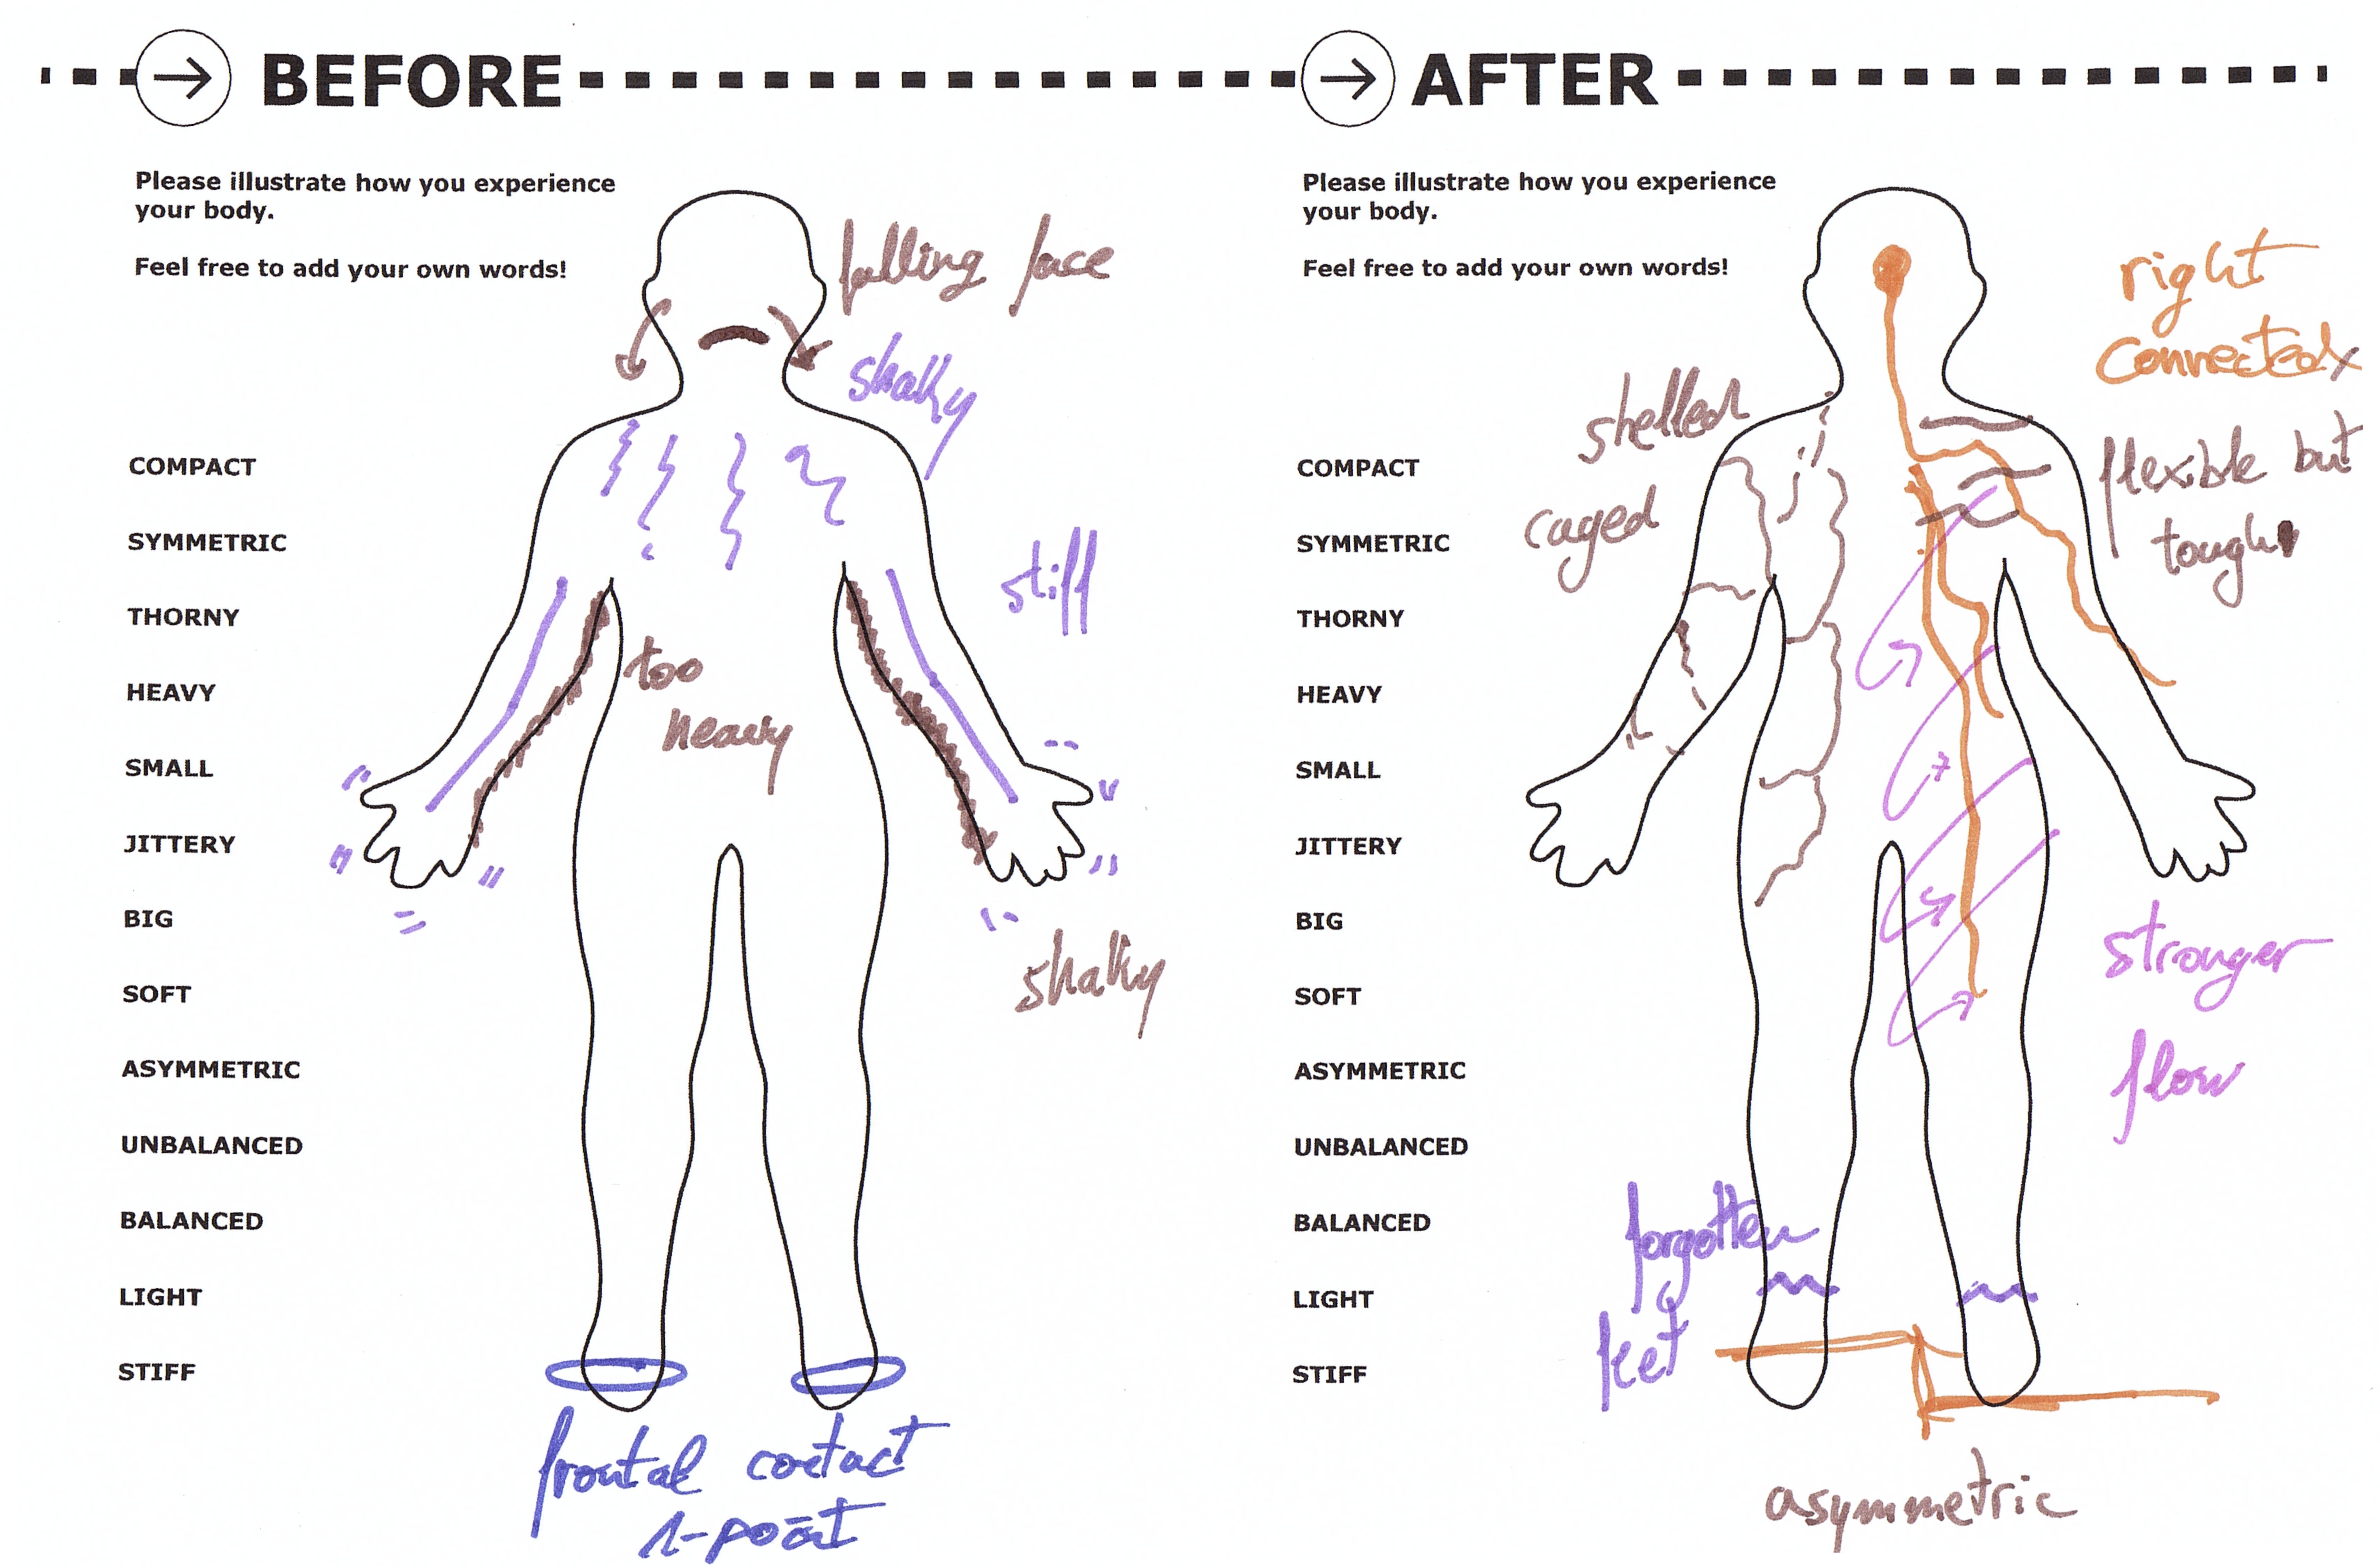
\includegraphics[width=0.95\linewidth]{Chapters/Figures/soma_chi/Bodysheet_highres.png}
  \caption{Example of a body sheet used to document the somatic experience during the design process}
  \label{fig:bodysheets}
%   \Description[From feeling shaky and stiff before the exploration to building an asymmetric awareness of the body]{A body sheet showing the changes of the somatic experience before and after a soma design workshop. Before, the participant felt shaky and stiff, aware of a heavy feeling in the arms and a single-point contact of the feet. Afterwards, the participant experienced an asymmetric awareness of the body: The left side felt caged, while the right side was more connected, flexible but tough, and with a stronger flow of energy. The feeling in the feet was forgotten after the workshop.}
\end{figure}

These sessions enabled the authors to narrow down the physical schematics that would facilitate meaningful interactions. They included a set of suitable pad shapes/sizes and bodily placements that could be embedded into a wearable interactive system.

\subsection{Autobiographical Design: First-Person Engagement with Shape-Changing Materials and Breathing}
\label{sec:first_person_engagement}

Based on the insights obtained during the soma design workshops, Annkatrin created a restrictive garment which contains the shape-changing pads, pressing against both the upper and lower back. It was inspired by the design of similar compression garments \cite{vaucelle_design_2009, foo_user_2019}, but not intended to represent a final design outcome nor a prototype for deep touch pressure therapy. Instead, the garment acted as an experiential artifact \cite{sundstrom_experiential_2011}, an intermediate tool in the design process to present new and interesting experiences and discover their affordances through embodied interaction with breathing-based deep pressure.

 \begin{figure*}[t]
  \centering  
    \includegraphics[width=0.8\linewidth]{Chapters/Figures/soma_chi/fig_5_all_grid.png}
  \caption{The garment, worn with a breathing sensor and one pad in each inner pocket}
  \label{fig:garment}
\end{figure*}

Figure \ref{fig:garment} shows the breathing garment being worn. A respiration sensor is strapped around the torso underneath the garment. On the inside, two pockets are attached on the upper and lower back. Each pocket holds one inflatable pillow to apply deep pressure on different areas of the back. When closed, the garment fits tightly and can transfer the deep pressure applied by the pads. The outer material can be closed in the front with a loop-and-hook fastener which allows for a tight fit in the torso area, making the actuation clearly noticeable. The pads can be placed in two pockets on the inside of the garment, one on the lower and one on the upper back. We would like to note that the garment needs to be closed to apply deep pressure and is left open in Figure \ref{fig:garment} to show the placement of the respiration sensor.

% During the exploration, the actuator devices were placed externally and connected to the pads in the garment via two elastic air hoses that are laced through a small hole at the bottom of the lower pocket. Although this constrained Annkatrin's movements within a small area around the actuators and required her to be careful when changing position, it did not detract from the interaction with the garment. The sound of the air pumps was dampened using noise-cancelling headphones playing white noise. 

% The garment was used along with an inductive respiration sensor to explore deep pressure feedback combined with different breathing techniques. The sensor was worn around the chest or stomach underneath the garment. Over the span of three weeks, Annkatrin conducted one to two sessions daily with a duration of 30-60 minutes each. These sessions were focused on exploring the potential impact of shape-changing deep pressure feedback coupled with a regular conscious breathing practice over a longer period of time on the subjective bodily experience and breathing awareness.

The sessions incorporated different breathing techniques as well as different contexts and positions, including lying on the back, sitting on a chair or doing other tasks such as reading or writing while wearing the garment. These positions and breathing patterns were informed by a two-months systematic exploration of deep pressure guiding different kinds of breath regulation, such as controlling the duration of inhalations and exhalations or alternating between diaphragmatic and thoracic breathing, done by Annkatrin in between the soma design workshops and the construction of the garment.

In total, four different breathing techniques were used: 
\begin{enumerate}
    \item 5.5 pattern: Providing a constant rate of 5.5 inflate-deflate cycles, i.e. breaths, per minute, which has been associated with increased heart rate variability and relaxation \cite{lin_breathing_2014} 
    \item Three-part breath pattern: This was inspired by the three-part breathing technique from yoga \cite{sengupta_dirga} which combines diaphragmatic and thoracic breathing. One pad is placed on the lower and one on the upper back. The one on the lower back is inflated first followed by the one on the upper back, guiding the user to first fill the stomach with air and then let it expand into the rib cage and chest. Then, the pad on the upper back is deflated again followed by the one on the lower back, guiding the user to release the breath first from the chest and then the stomach. Each inflation and deflation interval has a duration of 2 seconds, with a 1 second pause in between breaths. 
    \item Standardised feedback based on breathing sensor data with a 2 second pause in between breaths. It mirrors the user’s breathing intervals, multiplied by 1.7 to gradually increase the duration of one breath without making the difference between two successive intervals too large.
    \item Adaptive feedback with an actuation change triggered by rapid breathing. At baseline, the inflation speed is set to 50\% of the maximum, which makes the pads less noticeable. If the calculated inhale or exhale duration is shorter than 2 seconds, the inflation speed is increased to 100\% until the breath becomes longer again.
\end{enumerate}

At the beginning of each session, Annkatrin conducted a short body scan to take note of her present bodily sensations and breathing. Then, Annkatrin explored each combination of actuation pattern and position or context for at least 20 minutes before moving on to the next to experience more long-term effects of each condition. A single session was focused on a maximum of two different actuation patterns or two different body positions.

The exploration was documented in the form of an online diary as an intermediate step in the process of articulating the experiences. Initial impressions of the effects of the breathing exercises and the pressure feedback on the breathing and bodily experience as well as notable changes in the inductive respiration sensor data were noted down quickly and informally. As it was often difficult to articulate the primarily bodily explorations while still immersed in the process, it was necessary to take a short break afterwards before reflecting more deeply on the experiences based on the initial notes.

%%%%%%%%%%%%%%%%%%%%%%%%%%%%%%%%%%%%%%%%%%%%%%%%%%%%%%
%% EXPERIENTIAL AESTHETIC QUALITIES 

\section{Experiential Aesthetic Qualities}
\label{sec:aesthetic_qualities}

In the following, we present the four experiential aesthetic qualities that grew out of our design explorations. Such qualities bring out the aesthetic potential of interactions and how they are experienced in use \cite{lowgren_2009}, serving as an abstraction tool to articulate the insights which emerged over a series of explorations \cite{stahl_evocative_2014}.

Each quality is introduced with a body of examples that highlight how the quality manifested in different first-person interactions. In reflection of these accounts and the data collected in the design explorations, we then outline the aesthetic potential of shape-changing deep pressure feedback and the overall influence this had on different breathing techniques. We discuss how pressure-based feedback can be used to cultivate breathing awareness, appreciation, controllability and deconstruction. The different experimental configurations allowed us to document a range of experiences relating to our breathing patterns, some yielding a greater awareness by reinforcing our habitual behaviour, and others disrupting the familiar movements.
% 

\subsection{Placements on the Torso -- Symmetric versus Asymmetric}

Insights of the importance of symmetrical as well as asymmetrical feedback arose from how the inflatable pads could be moved around to different locations on the torso. This made it possible to put deep pressure on, for example, the back right shoulder at the same time as another inflatable put pressure on the lower left-side of the belly. By symmetrical feedback, we are referring to pressure applied equally on the left and right sides of the torso, i.e. symmetrical on the lateral plane with the same actuation pattern. Asymmetrical feedback refers to one-sided pressure or pressure on both sides of the body, but a) on different body parts or b) with different actuation patterns.


\subsubsection{Experiencing symmetric and asymmetric feedback}

The team's explorations naturally began with symmetrical placements, leading to a whole range of interesting experiences. For example, when Annkatrin was experimenting with placing the inflatable pillows symmetrically on both shoulders, as shown in Figure \ref{fig:neck}, position (1), she experienced massage-like qualities or "\textit{someone putting a comforting hand on your shoulder}”. When placing the pads near the lower back or waist area when sitting or lying down, the pressure created a sense of support and stability. This was especially pronounced when placing the pads on either side of the lower back in a lying position, forming "\textit{a small indent in the floor to enclose my body, causing a comfortable and safe feeling}." Annkatrin reported feeling unsteady and in lack of 'support' when the pillows were taken out or deflated, as if she would "\textit{roll to the left or right side at any moment}". The symmetrical placement of the pads under the body was often helping Annkatrin to "\textit{feel more connected to the floor, more grounded in my body and my environment}." Generally, interactions with symmetrical placements and patterns invoked calm and relaxed feelings: "\textit{I was left feeling much more in touch with my body, more calm and centred in myself. I felt loose, relaxed and a bit sleepy, similar to how I feel after a yoga practice or a good workout.}" 

Inspired by Feldenkrais exercises, Annkatrin, William and Miquel went on to experiment with asymmetrical actuation during the design workshops. Many Feldenkrais lessons aim to deconstruct the habitual coordination of movements. It is done in order to draw attention to their finer details or offer novel ways in which movement can be created, ultimately leading to alternative habitual movement patterns. Based on those Feldenkrais lessons, Annkatrin, William and Miquel tried to re-create a similar feeling of imbalance or deconstruction by placing the pillows on only one side of the body or putting two pillows simultaneously on different body parts. This created two different effects: while applying the actuation to two different body parts made it "\textit{hard for us to decide where to direct our attention which created an ill-fitting, incongruous experience}", concentrating on only one side of the body "\textit{allowed us to become more aware of how we experienced that specific body part}".

Later, Annkatrin continued to experiment with asymmetric actuation using two pads with conflicting or complementing rhythmic patterns at the same time. As opposed to random or conflicting feedback, we define \textit{complementing asymmetric feedback} as requiring a regularity of sorts: the actuation intervals of one pad can be a multiple of the second pad, or one pad inflates while the other deflates. A \textit{conflicting pattern}, on the other hand, has incoherent phases, switching from inflation to deflation at different times. These explorations revealed that "\textit{the placement of the pads had to be matched carefully to the actuation}" to avoid interfering with each other or with the user's breathing. In particular, conflicting asymmetric actuation was perceived as distracting and uncomfortable, not leading to any deeper engagements. For example, placing the inflatables on the back of the thighs or using two very distinct actuation sequences "\textit{failed to evoke any strong effect}". In some cases such placements could even lead to strong negative experiences, preventing learning. Placing the pads asymmetrically close to the neck, as shown in Figure \ref{fig:neck}, position (2), made Annkatrin feel "\textit{like I was not able to breathe properly}", evoking associations with "\textit{having a snake wrapped around my throat}". On the other hand, when the position and patterns were complementing -- for example, when Annkatrin tried putting two pillows with one inflating twice as fast as the other on the lower back (Figure \ref{fig:neck}, position (3)) -- they "\textit{created a very unusual twisting sensation in the torso}". This in turn lead to insights on how locally applied effects can spread across the entire body, and helped Annkatrin to experience how different parts of the body are connected into a whole. 

 \begin{figure}[t]
  \centering  
  \includegraphics[width=0.9\linewidth]{Chapters/Figures/soma_chi/fig6_positions_numbers.png}
  \caption{Applying symmetric and asymmetric deep pressure to the shoulders (1), neck (2) and lower back (3)}
    \label{fig:neck}
    % \Description[Applying symmetric and asymmetric deep pressure to the shoulders, neck and lower back]{Applying symmetric deep pressure to the shoulders, as well as asymmetric deep pressure to the neck and lower back. In the latter case, pressure is applied more strongly to the right side of the body.}
\end{figure}

\subsubsection{Reflecting on symmetric and asymmetric feedback}

Symmetry is represented in many different forms in the HCI projects focused on breathing. In  projects with visual feedback, symmetry has been expressed as: visualization of two living lungs \cite{abushakra_augmenting_2014}; symmetrical  geometrical figures \cite{van_rooij_deep_2016, prpa_hacking_2016} or living virtual structures \cite{patibanda_life_2017} located in the centre of the screen or virtual environment; or as abstract symmetrical visualizations taking the whole computer screen \cite{moraveji_breathtray_2012}. One can see symmetry expressed as varying light intensity in the Philips LivingColor pair of lights \cite{dijk_breathe_2011}. In the projects using vibration as output medium, symmetry is found in the relative position of the vibrating artefacts on the body, such as: centre of the belly \cite{bumatay_investigating_2017}; centre of the upper chest \cite{frey_breeze_2018}; or in the blanket that has the same vibro-tactile sensation on both sides of the body \cite{dijk_breathe_2011}. In projects using shape-changing actuation as a medium to display breathing, symmetry is found in: the equable expansion and contraction of a living wall \cite{sjoman_breathing_2018}; in dynamic building structures \cite{moran_exopranayama:_2016, schnadelbach_exobuilding:_2012}, as well as in the whole shape of a particular probe \cite{aslan_hold_2016, kim_breathingframe_2015}; or sometimes experienced by the whole body symmetrically \cite{sun_breath_2017}. 

 \textit{Asymmetry} as a design quality of breathing feedback has not been explored as much. There have only been a few asymmetrical representations, such as a visualization of tides in the virtual garden \cite{roo_inner_2017}, and a few examples of providing direct feedback onto only one side of the body, such as the guiding shape-changing pillow under the right palm of the hand in the works by Yu and colleagues \cite{yu_breathe_2015}.

The focus on symmetrical representations in design work may be rooted in the notion that symmetry is commonly associated with perceived beauty and satisfying aesthetic experience \cite{nadal_study_2020, mcmanus_symmetry_2005}. Well-balanced presentations of equal proportions are more compatible with classical mathematical structures, and the link between symmetry and beauty even has explicit associations with our biological presence \cite{cardenas_symmetrical_2006}. However, absolute symmetry is not something we normally experience in the natural world, and leaves insufficient space for unpredictability and thereby discovery \cite{mcmanus_symmetry_2005}. We also note that the idea that symmetry is aesthetically pleasing is more prevalent in western culture \cite{nadal_study_2020, zeki_clive_2013}

While we might perceive a human body as symmetrical when we compare our left half to our right half, it is obviously not. All the projects mentioned above in some way or other represent the lungs as a system with the perfect bilateral system. However, in a healthy individual, the left lung is slightly smaller than the right one to make some space for the heart -- as the heart is slightly shifted to the left. Our limbs are also asymmetric, often making one side of our body the more dominant one. Some of us are writing with our right hands, some with the left, and even ambidextrous people find it hard to use both hands for every habitual task. Our limbs are not perfectly equal -- there is often a limb length discrepancy. We are asymmetrical by nature and through training and everyday habituation, we might become even more asymmetrical in ways that harm us.

What then is the aesthetic potential of addressing these asymmetries in design? While symmetry and symmetrical feedback is a well-explored and articulated quality and approach, proven to be beneficial for creating feedback that is easy to grasp and follow, asymmetry has not been explored as much. What we found is also how asymmetrical feedback can be quite unpleasant and distracting. But when designed carefully, it can be very informative for the design process -- as well as to users aiming to increase their breathing awareness. What is sometimes needed is a journey from asymmetry to putting those asymmetrical experiences back into a symmetric whole, as is often done in Feldenkrais exercises. For example, we might want to address the diagonal connection from the left lung into moving the hip on the right side, and then the connection from right lung to left hip movements, but then we need to put both together in order to explore and feel how all these parts are interconnected. If we leave the user with only one half of this experience, for example the connection from left lung to right hip, they might leave the exercise with a feeling of being lopsided. 

Asymmetry as a quality is widely used in Feldenkrais practice for disrupting the processes of the familiar \cite{worth_symmetry_2015}. In Feldenkrais lessons it is achieved by directing attention to just one side of the body, one lung, particular limb or other body part. This allows us to break the circle of habitual experience and reconstruct them bit by bit, slowly and attentively into something new -- evocative and unusual. 

\subsection{Guiding Different Kinds of Breathing}

There are many possible breathing patterns promoted by different physical disciplines and body practices. Some are specifically targeted at focusing the mind and increase bodily awareness \cite{kupershmidt_definition_2019, burke2008role}. To further explore the different muscles and bone structures involved in breathing, we decided to more deliberately impose deep pressure on different locations of the breathing apparatus in a manner that mirrors and encourages these different breathing patterns.  

\subsubsection{Experiencing breathing in different body parts}
Applying deep pressure to different locations on the body not only made it possible to explore symmetric vs asymmetric feedback, but also to feel the breathing in different body parts. The actuation was adapted to the user's breathing by inflating the pillows during inhalation and deflating the pillows during exhalation, including a slight delay as the user’s breathing intervals are computed from sensor data. This interaction is from here on referred to as \textit{following} the user's breathing.

The explorations started with taking conscious breaths through the chest while placing the inflatable pillows on and under different body parts which revealed their potential to physically move the body in certain directions. This led to a range of interesting experiences that were not necessarily related to breathing, such as placing them under the feet to cause a movement which Annkatrin related to "\textit{walking on the spot.}" 

However, Annkatrin experienced breathing-based actuation mirroring her breathing on the lower body as "\textit{uncomfortable and unnatural since I could not relate those body parts to my breathing}", which made her feel "\textit{weird, like it's not supposed to be there}". Instead, the pressure was more readily associated with breathing when it was applied close to the breathing apparatus, i.e. on the torso or upper body. Annkatrin associated forward and upward movements of the torso with an inhalation, "\textit{the pads seemed to push me to inhale}", while moving backwards and pressing down on the torso were perceived as an exhalation. Placing the pads underneath each armpit "\textit{pushed my arms away from the body}", creating a feeling of the chest expanding during an inhalation. In this way, the pressure was able to support certain ways of breathing by reinforcing the respective movements. Annkatrin found that when the pads were placed under the lower back, the pressure "\textit{encouraged me to breathe more with my stomach}", while placing the pads on the upper back "\textit{made me breathe more with my chest.}" Guided by the pressure, Annkatrin was able to learn how to engage different muscles when inhaling and thus practice diaphragmatic or thoracic breathing.

To investigate these different breathing patterns further, Annkatrin, as well as Pavel and Kia in their explorations, created an actuation pattern based on the three-part breath, a technique from yoga practice which combines diaphragmatic and thoracic breathing in each inhalation and exhalation. Since this exercise requires a certain amount of awareness and control over which muscles are engaged when breathing, Annkatrin had to "\textit{focus a little more to direct my breath from my stomach to my chest and back.}" With one pad placed on the upper and another on the lower back however, she reported being able to follow the guidance of the deep pressure "\textit{without having to think about how I was supposed to breathe.}"

Over time, the exercises created a lasting effect which carried over into Annkatrin's everyday life: "\textit{I could feel the muscles in my torso more distinctively when walking around. I was experiencing my breathing more intensely throughout the day, leading me to take deeper breaths than before and use my stomach and chest more deliberately and distinctly while breathing.}". This suggests that by applying deep pressure on certain body parts, the pads may help improve someone's control of their breathing over time, stimulating engagement with certain muscles to assist different ways of breathing with regular practice. While three-part breathing is just one possible option, a plethora of techniques exist, such as letting the rib cage expand towards the arms, chest, back or shoulders when inhaling. Each of these directions engages different muscles around the rib cage, that, when trained, can open up a rich repertory of breathing techniques. 
% 

\subsubsection{Reflecting on different kinds of breathing}

While many different muscles and bone structures are involved in breathing and enable distinct breathing patterns, breathing-based designs have mainly focused on reducing users' breathing rate \cite{prpa_inhaling_2020}. Whilst some of these studies account for lung capacity (e.g \cite{abushakra_augmenting_2014}), attention towards individual breathing muscles is normally ignored, neglecting the opportunity to practice alternative breathing patterns using these muscles.

Only a few breathing-based designs employ different types of breathing, for example encouraging deep diaphragmatic/abdominal breathing to alleviate stress \cite{prpa_hacking_2016} and anxiety conditions \cite{van_rooij_deep_2016}. Others measure breathing on different body parts \cite{prpa_attending_2018}, taking into account diaphragm expansion \cite{desnoyers-stewart_jel:_2019} as well as the rising and falling extent of the abdomen \cite{schnadelbach_exobuilding:_2012}. 

Outside of HCI, a handful of studies validate the use of additional sensor placements in order to differentiate between thoracic and abdominal breathing, such as the work by Hamnvik and colleagues on Yolo4Apne \cite{hamnvik_yolo4apnea_2020} which uses two inductive respiration sensors and \cite{ejupi_detection_2018} that uses three resistive stretch sensors across the torso. This approach has shown to be effective in extending measurement potentials, but it does not address alternative representations or interactions to guide users to explore novel breathing patterns.

So far, the interactive systems for breathing guidance do not reflect the immense resources we have for breathing, not only in regards to muscle engagement but also inhalation and exhalation sequences. Instead, breathing is often reduced to a single dimension that only operates from one part of the body, without registering these anatomical intricacies. What then are the technological interventions that may facilitate a richer breathing experience?

Though not extensive, three generic descriptors (clavicular, thoracic, and diaphragmatic \cite{rama_science_1998}) provide a starting point to distinguish types of locational breathing. These also provide the foundation for the three-part breath technique (also known as Dirga Pranayama), which has been thoroughly studied in traditional yoga practice \cite{sengupta_dirga}. It demands specific attention to separate parts of the breathing apparatus, namely the abdomen (lower torso) and thorax (upper torso), and considers how these are used in conjunction to expand breathing capacity through \textit{full} and \textit{complete} breaths, compared to chest-based breathing.

However, there are many other breathing practices, such as those employed by professional singers or dancers, offering hitherto unexplored potential to provide engaging interactions. The way in which we breathe has a direct impact on the body's chemical makeup and behaviour of the autonomic nervous system \cite{russo_physiological_2017}. Moreover, it is widely recognised that longer breaths incorporating the whole body can lead to improved overall well-being in the long term, particularly in regards to stress regulation \cite{moraveji_peripheral_2011}. Studies of alternative breathing patterns suggest that by engaging individual muscles and body structures, we can train ourselves to gradually gain greater awareness and control of our holistic body \cite{van2007whole}.

There exists a multitude of possibilities when it comes to engaging with breathing, and the same goes for halting the breathing. One can pull air into the lungs using the diaphragm or muscles in the neck, let the rib cage expand towards the back or the shoulders, and stop the breathing by pulling down the diaphragm, pushing the stomach out or tensing muscles around the rib cage. Many combinations of these techniques are possible, and can be further combined with other movements such as tensing or relaxing the pelvic floor. All add to the richness of the experience.

Thus, our explorations point towards a potential for interactions which incorporate a richer catalogue of breathing methods, creating the need to measure movements on different parts of the body to differentiate between small muscles involved in breathing. But the breathing rhythm does not consist of one-off breaths; instead, it is a pulsating, vibrant flow that engages a variety of muscles and body structures over time. This raises new questions as to how a system can turn a series of breaths into a malleable and adaptive rhythm, allowing the user to engage with their breathing pattern over an extended period of time.


\subsection{Synchronous vs Asynchronous Feedback}

By \textit{synchronous} feedback we are referring to deep pressure that follows the user's breathing rhythm. \textit{Asynchronous} feedback, on the other hand, provides a rhythm that is slightly or entirely out of phase with users' breathing, at times even pushing back right when the user inhales and expands their stomach or chest and vice-versa.

\subsubsection{Experiencing synchronous and asynchronous feedback}

At first, the explorations during the design workshops were focused on synchronous feedback, using actuation patterns which imitated the user's own breathing rhythm. These generally felt comfortable and supportive. The deep pressure drew attention to the breathing by making the breathing intervals more tangible and apparent, allowing Annkatrin to "\textit{appreciate my body and its ability to breathe steadily}". The synchronous feedback also created an interesting interplay when sitting on a chair, since leaning back on the pads made the changes in pressure and thus the chest movements more intense, letting the entire body sway back and forth in the breathing rhythm. As the pads were physically pushing the body forwards to support inhalation, Annkatrin reported feeling like "\textit{they were in charge of my breathing and I could let myself surrender my control over my breathing to them}", eliciting a sense of intimacy and safety.

Even when the actuation was not based on breathing sensor data but rather on pre-programmed sequences, Annkatrin, William and Miquel tried to match their breathing to the inflation and deflation of the pads. The pressure was not noticeable during the shift from deflation to inflation, which made Miquel feel "\textit{lost till I realised I should have been inhaling already}", whereas Annkatrin felt "\textit{like I was not supposed or allowed to breathe}" and thus held her breath until the pads began to inflate. Not being able to follow the rhythm set by the pads, which occurred for example when the intervals were very long, evoked feelings of guilt and frustration.

Pavel and Kia reported on similar experiences of frustration. Kia in particular found that for certain breathing exercises, she felt pressured to perform and when she could not adhere to the requirement, she felt as if the system was trying to discipline her. For example, she tested "square breathing" -- a method where you are asked to breathe in while counting to five, hold your breath while counting to five, breathe out while counting to five and then hold your breath again, and then increase the counting, for example, up to 10. The method is quite demanding. It helps train stamina and breathing ability for professional singers. The experience of being 'controlled' by the system became too strong for her when she did square breathing with the system.   

Annkatrin, William and Miquel purposefully experimented with asynchronous patterns by using two inflatable pillows with conflicting patterns at the same time, inflating and deflating them in opposite or completely unrelated rhythms. Similar to asymmetric actuation, these patterns had to be crafted carefully to make sure that actuation sequences which were used simultaneously did not actively work against each other. Otherwise, they were dismissed as "\textit{hindering and annoying}", such as when one pad was supporting inhalation by inflating while the other was discouraging it by deflating. At times, the asynchronicity also created unpleasant experiences, like feeling "\textit{dizzy or sea-sick}" when using an asynchronous pattern which inflated one pad while deflating the other and vice versa while lying on the back.

Annkatrin noted that when the pads were contradicting each other or the natural flow of breathing, following their guidance felt like working against the body instead of engaging with the body. Switching the two pads during the three-part breath pattern, were guiding Annkatrin to first breathe in with the chest and then with the stomach. "\textit{This way of breathing made me feel like I was not getting enough air, thus appearing forced and unnatural.}" Annkatrin also reported finding it difficult and uncomfortable to breathe in an asynchronous rhythm, for example by holding her breath or taking intentionally short breaths. "\textit{Not following the pads seemed wrong since I was not engaging with my body but closing myself off to my body.}"

However, when all aspects complemented each other, the asynchronicity of the feedback was able to provoke interesting and unexpected experiences. The pads were generally seen as a "\textit{small extra pair of lungs}", connecting inhalation to inflation and exhalation to deflation. To reverse this more familiar way of breathing, Annkatrin tried placing the pads on the stomach. This forced her to breathe in the opposite way, taking the pressure caused by the inflation as a cue to exhale and letting deflation make room for the stomach and chest to expand during inhalation. While such a breathing pattern accommodated the pressure on the stomach in a way that allowed Annkatrin to take deep breaths, it "\textit{required much more concentration because it was different from every other pattern I had tried so far}". She had to figure out how to adapt to the pressure to be able to accommodate the pads and breathe comfortably, which made the pads seem like they were "\textit{restricting and controlling my breathing}". Thus, the pressure forced Annkatrin to breathe very deliberately and thoughtfully, "\textit{drawing my attention to the mechanics of breathing and re-evaluating the pads’ connection to my breathing}". When used in this way, the asynchronous actuation was able to deconstruct breathing, creating the challenge to become comfortable with being thrown out of rhythm.


\subsubsection{Reflecting on synchronous and asynchronous feedback}

Synchrony is a quality that takes different forms in breathing-based design projects. The most straightforward is a direct mapping of a user's breathing pattern to certain feedback from the system. This is mostly done in phase, mapping expansion to inhalation and contraction to exhalation, with the exception of a photo frame that inflates when a remote person exhales and vice versa \cite{kim_breathingframe_2015}. The inhalation has been mapped to many different output modalities, including the expansion of a visualised geometrical shape \cite{van_rooij_deep_2016, prpa_hacking_2016, wongsuphasawat_you_2012} or pair of lungs \cite{abushakra_augmenting_2014}, tides in a virtual environment \cite{roo_inner_2017}, an increase in light intensity \cite{dijk_breathe_2011, stahl_soma_2016}, as well as the expansion of a physical artefact \cite{aslan_hold_2016, kim_breathingframe_2015, sun_breath_2017, moran_exopranayama:_2016, sjoman_breathing_2018}. Breathing phases can also be tied to the directions of movement of the protagonist in a video game \cite{sonne_chillfish_2016} or of the user in a virtual environment \cite{van_rooij_deep_2016, davies_osmose:_1996, prpa_hacking_2016}.

Synchrony may also involve more elaborate forms of feedback. When the user has fallen out of sync with the system, for example by breathing faster, the system can provide a guiding rhythm in form of vertically moving on-screen elements \cite{moraveji_peripheral_2011} or pulsating video and audio signals \cite{ghandeharioun_brightbeat_2017}. In multi-user systems, synchronous breathing of several users can make a sponge grow in a virtual environment \cite{desnoyers-stewart_jel:_2019} or trigger light effects on a garment worn by one of the users \cite{schiphorst_breath_2006}. 

Asynchronous feedback can take form of shaping a soundscape based on different attributes of participants' breathing \cite{vidyarthi_sonic_2012}, as well as receiving instructions from a virtual breathing coach to modify the breathing rate without specifically addressing the user's actual breathing cycles ("continue breathing at a slower pace”) \cite{shamekhi_breathe_2018} or showing the current breathing rate as a percentage of the individual resting breathing rate \cite{moraveji_breathtray_2012}. Asynchrony is also used in various negative feedback loops, in which a fast breathing rate increases the difficulty of a video game \cite{chill-out_2014} or amusement ride \cite{marshall_breath_2011}, or lowers the quality of a song played in the background \cite{harris_sonic_2014}.

However, the majority of breathing-based systems reported in the literature encourages synchronous breathing patterns, aiming for synchronous feedback in harmony with the user's breathing rhythm. This is not surprising, as similar to symmetry, synchrony is an integral construct in technology, finance, molecular biology, physics, music and psychology which indicates coordination patterns among processes as well as precise coincidence of events in time \cite{ravignani_2017}. Rhythm is one of the most important pillars of contemporary music, enabling the singers and musicians to not lose themselves in the music and stay in sync: one may miss a tone, but missing the rhythm can deteriorate the perception of the entire piece \cite{levitin_this_2019, reich_writings_2004}. Nevertheless, a well-executed asynchronous element -- syncopation, which is a deviation from an expected rhythmical pattern -- enriches the piece and may bring listeners enjoyment and a desire to move \cite{sioros2014syncopation}. Moving away from music, where tones are coherent and concurrently executed, language is also performed in antiphony as individuals take turns in conversations \cite{ravignani2014chorusing}. If we regard breathing as a dialogue between the system and the user, asynchronous forms of feedback can open up a new design space for deeper and more elaborate forms of interaction. Similar to asymmetry, careful and deft application of asynchronous elements in breathing feedback may break the patterns of habitual perception of breathing and make us more self-aware. 
We recognise that it sometimes takes time and effort to learn a difficult breathing practice, but still, it is important that the user does not lose faith in their ability along the way. There needs to be a path towards overcoming the uncomfortable experiences through practice, step by step learning more and more, but not demanding too much too soon. 

\subsection{Breathing Correspondence: Finding a Balance between Leading and Following}

The findings made us think that a really interesting dialogue between the system and the user could be achieved, a dialogue that would rely on both letting users express their breathing, but at the same time being influenced, through feedback, encouragement or even strong pressure. We therefore continued to explore exactly how to find a balance point right between \textit{leading} and \textit{following} breathing patterns by first applying deep pressure -- almost to the point of being unpleasant -- and then releasing in rhythmic flow. We will refer to this experience as a \textit{breathing correspondence}. 

\subsubsection{Experiencing different roles in the interaction}

The explorations of different actuation patterns revealed how the inflatable pads could take on different roles in the interaction. If the actuation was following a predefined rhythm independent of the breathing sensor data, it was more likely to be perceived as not engaging in dialogue or adapting to the user, but instead leading the interaction and providing breathing instructions. They seemed to be "\textit{guiding or even steering the breath}", reinforced by the pressure physically pushing the body forward.

When the actuation was based on the breathing sensor data, the pads assumed a more passive role in the interaction by following the user’s breathing. In turn, this gave the user a more active role, allowing them to deliberately breathe in a different rhythm in an attempt to control or influence the pads. For example, during the design workshops Annkatrin, William and Miquel experimented with holding their breath and manipulating the length and depth of their inhalations and exhalations. Annkatrin reported having "\textit{the impression that the pads were listening to me which created a sense of intimacy and safety, like the pads were taking care of me}". Such semi-autonomous interactions created an interesting contrast between breathing “with” the pads when following along to the actuation pattern and breathing “against” the pads when trying to change the pattern. However, it was not always clear whether the pad was adapting to breathing or vice versa, which introduced a sense of ambiguity in the interaction.

This potential for ambiguity motivated further attempts to combine both a leading and a following role in a single actuation pattern by extending the breathing feedback by different factors. We made it possible to influence the actuation by manipulating the breathing while the pressure was at the same time influencing the user to gradually take longer breaths. A dialogue between the system and the user emerged, using the pads as a communication channel: "\textit{As the pads were mirroring my breathing intervals while pushing me to gradually extend my breath, I was trying to match my breathing to the actuation, feeling the changes reflected by the pads.}"

The deep pressure becomes stronger with each interval almost to the point of being unpleasant, pushing Annkatrin to "\textit{take an excessively deep breath completely filling my lungs with air to the point of discomfort}". Right before the pressure starts to become painful, it is released in a rhythmic flow, prompting the exhalation as a "\textit{sigh of relief}". As the pressure intensifies and fades away gradually while providing a constant presence, it serves as a constant reminder to attend to the breath. The breathing feedback allowed Annkatrin to "\textit{become more aware of unintentional changes and try to make sense of them. For example, struggling to extend my breathing intervals made me wonder whether I was stressed or worried about something and therefore unable to take deep breaths.}" The pads were perceived as an extension of the physical self rather than an external influence, allowing Annkatrin to "\textit{engage in a dialogue with my body, not just the system itself.}"

However, when this balance between leading and following was disrupted, the pads began to dominate the interaction. After Annkatrin incorporated a threshold which increased the actuation speed and thus the pressure when the breathing intervals fell below two seconds, the experience changed significantly: "\textit{I was constantly aware of the pads and the pressure, trying to identify the current actuation speed and keep my breathing intervals above the threshold}". Feeling the intervals become longer evoked a sense of accomplishment, while feeling them become shorter caused guilt and frustration which put Annkatrin under stress to extend her breathing. "\textit{It was a relief to take off the garment because I no longer felt pressured to actively control my breathing}". Such exploration of the tipping point between leading and following can provide insights on how gradual pressure changes help to achieve a harmonic interaction, while strong or sudden changes are perceived like a firm command, taking over the control of the interaction.

Further explorations showed that just sitting with the pressure and breathing in one's own rhythm, neither trying to follow nor influence the actuation, could also create interesting experiences. In such interactions, the pads assumed the role of a companion which provided a "\textit{soothing sense of presence, like there was another person sitting next to me and sharing their breath with me}". The pressure was not distracting, but rather seemed to complement one's individual breathing rhythm. Annkatrin reported that experiencing the pressure in the background while working led her to "\textit{take deeper breaths subconsciously without making an effort to do so}".

Kia reported similar experiences -- feeling that she could accept the system more willingly if she just let it act in the background while she was working away on her computer. Whether she was in fact following the feedback from the system or not became unimportant and she could relax into the experience. 

\subsubsection{Reflecting on establishing a breathing correspondence}

According to their role in the interaction, breathing-based designs can be split into two distinct strands: in the Self - System - Self modality \cite{prpa_inhaling_2020}, the system is following the user's breathing pattern \cite{abushakra_augmenting_2014, sonne_chillfish_2016, bingham_breath_2010, roo_inner_2017, prpa_hacking_2016, shaw_meditation_2007, aslan_hold_2016, pisa_towards_2017, sjoman_breathing_2018, moran_exopranayama:_2016}, whereas in the System - Self - System modality \cite{prpa_inhaling_2020}, the user is following the pattern provided by the system \cite{wongsuphasawat_you_2012, yu_breathe_2015, soyka_enhancing_2016, dijk_breathe_2011}. Looking at the prevalence of the two strands among HCI projects, the majority of breathing-based systems belong to the first group, providing a mere representation of the user's breathing pattern of the user and in the process taking the role of a passive follower. Only a few systems take a leading role in the whole dialogue \cite{wongsuphasawat_you_2012, yu_breathe_2015, soyka_enhancing_2016} or one of the interaction modalities \cite{bumatay_investigating_2017, patibanda_life_2017}, providing users with a signal to follow. Despite the simplicity of the latter, it has proven to be a powerful interaction modality. Regardless of whether the user follows the interaction precisely or just leaves it as a peripheral stimulus, the interaction can provoke a relaxing and calming sensation when experienced for a prolonged period of time. This is also supported by the studies of Moraveji et al. \cite{moraveji_peripheral_2011, moraveji_breathtray_2012} showing the effectiveness of peripheral respiratory feedback on inducing a slower breathing rate without explicitly promoting focus on breath pacing or distracting users. 

Some breathing-based systems make the distinction between leading and following more ambiguous by taking users' natural rhythm as a baseline, then feeding it back to them at a slightly slower pace to guide them to gradually extend their breathing \cite{moraveji_peripheral_2011, ghandeharioun_brightbeat_2017}. While this is a form of biofeedback aimed to achieve optimal HRV readings and supported by several studies \cite{vaschillo_characteristics_2006, steffen_impact_2017, sutarto_resonant_2012}, HRV can be misleading when misinterpreted or interpreted in a shallow sense \cite{hrv_cammann_2002}. 

The concept of correspondence proposed by Ingold \cite{ingold_being_2011} and further adapted and reworked into \textit{intimate correspondence} by Höök et al. \cite{hook_somaesthetic_2016} calls for designing an interaction wherein the roles of leader and follower are unclear, the boundaries between user and system become dissolved and they start acting together as 'one'. This creates a more evocative communication to take form implicitly as there is no need to actively reply to the system's query -- a correspondence relationship where users' breathing is simultaneously influencing and being influenced by the system. 


%% DISCUSSION /CONCLUSION
\section{Discussion and Conclusion}
Through a first-person felt engagement over a longer time period, we uncovered several, previously unexplored breathing experiences spurred by different pressure patterns on the torso such as: 
\begin{enumerate}
    \item imposing symmetrical and asymmetrical pressure as a path to draw attention towards different  parts of the breathing apparatus, as well as spurring novel sensations by deconstructing habitual coordination of movements 
    \item the sequencing of inflation/deflation in accordance with the user's engagement with different muscles when breathing, leading up to more intricate breathing practices
    \item providing synchronous or asynchronous feedback via rhythmic pressure that is in sync, slightly or entirely out of sync with users' breathing rhythm as a step towards deepening aesthetic appreciation and increasing awareness of possible breathing rhythms
    \item exploring the balance point between influencing and simply following the rhythm of the user’s breathing -- constituting a breathing correspondence experience where it is unclear whether the system or the user is driving the breathing rhythm 
\end{enumerate}

We want to emphasise that while our explorations were inspired by deep pressure therapy, the design space we opened also points to other experiences and needs beyond delivering calming and relaxing effects. Deepening users' appreciation of their own breathing can be an aesthetically interesting experience in itself. Breathing provides a rich inner universe where different body parts such as the lungs, rib cage, posture, bone structures and fascia are intricately connected in ways that can be more or less 'known' to us depending on how bodily aware we are. Different muscular tensions, engaging in habitual as well as non-habitual ways of breathing, can relate to or even spur emotional experiences in the short-term. Apart from the experience in the moment, the lingering effects after a session, feeling like you have had an 'inner' massage, as well as potential long-term lasting transfer effects into everyday life situations are particularly intriguing to explore further. 
 
Apart from breathing guidance, pressure-based feedback may also be used on other parts of the body. By exploring experiences that breach into the domain of discomfort, we can begin to determine an appropriate equilibrium that lies between between gentle/subtle and uncomfortable/unpleasant \cite{benford2012_uncomfortable}. We show how discomfort can be imposed by increased intensity of actuation, irregular and asymmetrical positioning of the pads, along with asynchronous inflation patterns that go against users' natural, unreflected breathing. When the interaction is engaging with the non-habitual, the system may elicit conscious physiological reactions, requiring users to be very much present with their breathing. However, if this intensity goes beyond a certain threshold, we lose this relationship and the experience becomes meaningless or even unsafe. 

While we did not study social communication here, we know that learning to control our own breathing apparatus may also lead to better control over what we communicate to others. For example, consciously breathing in rhythm with someone else can lead to better communication and empathy \cite{keller2014rhythm}. Many body practices, such as improvisation dancing or martial arts, require coordinating breathing patterns not only with our own movements but also the person we are moving with \cite{codrons2014spontaneous}. 

Finally, we would like to point to how our first-person engagement turned out to be highly generative in terms of bringing out many design ideas for shape-changing materials applied on the torso. While more studies are needed to shift our subjective, personal understanding into reliable breathing engagements for larger user groups, our results show that first-person engagements will be one path to designing aesthetically rich, haptic engagements with shape-changing materials. This said, we are fully aware of the potential pitfalls of autobiographical design: the risk of designing only for the few people involved in the design process, ending up with designs that are irrelevant or even harmful to the targeted end-user group. The work we did here must be complemented with further design explorations, specifically aiming at different user groups, involving them in the design process. But as pointed out by Höök and colleagues \cite{hook_embracing_2018} "this felt
dimension, despite its subjective nature, is what provides rigour and structure to our design research". That is, the authenticity of the experiences we report on above relies on the long-term, deep, felt engagement of the designers -- a rigour of a different ilk. 

In summary, taken together, these first-person material explorations engaging with deep pressure feedback using shape-changing actuation managed to open a rich, somaesthetically evocative design space. We uncovered new paths of utilizing pressure-based feedback to cultivate appreciation, awareness, controllability and deconstruction of breathing, ultimately converging to an intimate relationship between system and user -- a \textit{breathing correspondence}.